\section{Implementación}

La implementación se desarrolla en etapas:

\begin{itemize}
    \item \textbf{Estructuras de datos:}
    \begin{itemize}
        \item Uso de grafos para modelar las relaciones entre usuarios.
        \item Implementación de listas enlazadas y tablas hash para gestionar datos asociados a cada usuario.
    \end{itemize}

    \item \textbf{Algoritmos:}
    \begin{itemize}
        \item Cálculo de la similitud de Jaccard para sugerencias basadas en intereses comunes.
    \end{itemize}

    \item \textbf{Manejo de datos:}
    \begin{itemize}
        \item Almacenamiento estructurado en directorios para cada usuario.
        \item Archivos separados para guardar seguidores, seguidos y datos generales de los usuarios.
    \end{itemize}

    \item \textbf{Generadores dinámicos:}
    \begin{itemize}
        \item Creación automática y controlada de usuarios.
        \item Generación de conexiones aleatorias y recomendaciones personalizadas.
    \end{itemize}

    \item \textbf{Interfaz de interacción:}
    \begin{itemize}
        \item Desarrollo de una interfaz de línea de comandos para manejar la creación, modificación y búsqueda de usuarios.
        \item Ejecución a través de parámetros para una interacción dinámica.
    \end{itemize}
\end{itemize}

\subsection*{Cálculo de la Similitud de Jaccard}

\begin{itemize}
    \item Para la implementación del índice de Jaccard, se utilizó una tabla hash para las representar las preferencias de cada usuario. Esto maximiza la eficiencia al realizar comparaciones necesarias entre las preferencias de dos usuarios y facilita el cálculo de dicho índice.
\end{itemize}

\subsection*{Creación Automática de Usuarios}

\begin{itemize}
    \item Para la creación automática de usuarios, se creó un modelo matemático que calcula la máxima cantidad de usuarios que podrían crearse según el número de perfiles en la red. Cada cierto intervalo de tiempo, se verifica el número de usuarios en la red y, en base a eso, se calcula la máxima cantidad de perfiles utilizando el siguiente modelo:
\end{itemize}

\[
U_{\text{máx}}(n_0) = \left(\frac{n_0 + 180}{n_0}\right)^{\frac{2}{3}}
\]

donde:
\begin{itemize}
    \item $U_{\text{máx}}$ es la máxima cantidad de usuarios.
    \item $n_0$ es el número de usuarios actual en la red.
\end{itemize}

Después de usar el modelo matemático para limitar la cantidad de usuarios que se puedan crear, se genera un número aleatorio entre \( 0 \) y el valor devuelto por la función. Este número representa la cantidad de usuarios a crear.

\subsection*{Justificación del Modelo Matemático}

\begin{itemize}
    \item El modelo matemático simula el crecimiento controlado de la red social, asegurando que cuando la cantidad de usuarios en la red alcance o supere los \( 100 \), solo se pueda crear un usuario nuevo a la vez. Esto permite que la red crezca de forma continua, pero cada vez más suave.
\end{itemize}

\begin{figure}[h!]
    \centering
    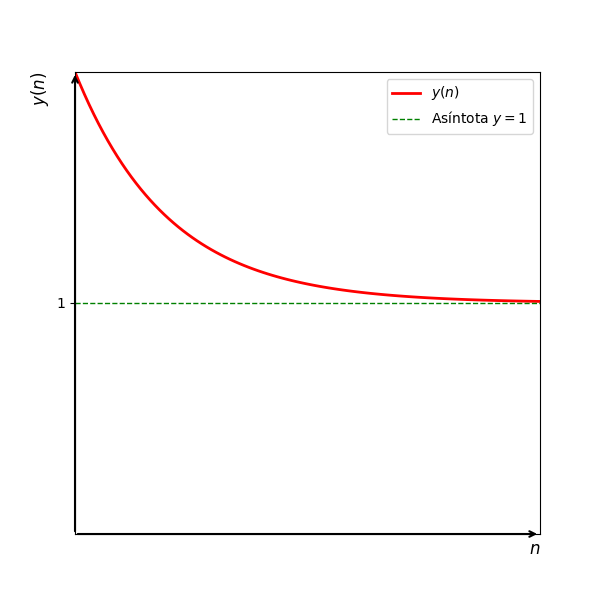
\includegraphics[width=0.5\textwidth]{src/figures/Figure_1.png}
    \caption{Ejemplo.}
    \label{fig:jaccard}
\end{figure}



La creacion del mdoelo se puede explicar en las siguientes expresiones matematicas, en dodne podemos observar el por que esta Modelo toma los comportamientos indicados anteriormente.
\begin{equation}
    \underset{n \to \infty}{\text{Lim}} \quad y(n) = 1 \quad (\text{Asintota horizontal en } y=1)
    %\lim_{n \to \infty} y(n) = 1 \quad (\text{Asintota horizontal en } y=1)
\end{equation}

\begin{equation}
   \left. \frac{dy}{dn} \right|_{n = m} < 0 \quad \forall  m \in \mathbb{R}^+ \quad \text{(Decreciente)}
\end{equation}

\begin{equation}
  U_{\text{máx}}(n) = \left\lfloor y(n) \right\rfloor \quad \text{(Discretizacion del modelo)}
\end{equation}



